\documentclass{article}
\usepackage{amsmath,amsthm,amsfonts,amssymb,amscd}
\usepackage{fullpage}
\usepackage{lastpage}
\usepackage{enumerate}
\usepackage{fancyhdr}
\usepackage[percent]{overpic}
\usepackage{mathrsfs}
\usepackage{wrapfig}
\usepackage{multirow}
\usepackage{amsmath}
\usepackage{amssymb}
\usepackage{amscd}
\usepackage{lscape}
\usepackage{graphicx}
\usepackage[usenames,dvipsnames]{color}
\usepackage{listings}
\usepackage[usenames,dvipsnames,svgnames,table]{xcolor}
\usepackage[left=2cm,right=2cm,top=2.5cm,bottom=2.5cm, headsep = 0.9cm]{geometry}
\usepackage{verbdef}
\setlength{\parindent}{0.0in}
\setlength{\parskip}{0.0in}
\usepackage{setspace}
\definecolor{gray}{RGB}{90,90,90}
\usepackage[colorlinks=true, linktoc=all, linkcolor=blue]{hyperref}
\usepackage{fancyvrb}
\usepackage{booktabs}
\pagestyle{plain}
\setlength\parindent{20pt}
\title{Building an R Package in Windows}
\author{Brian D. Williamson\\PhD Student, University of Washington Department of Biostatistics}
\begin{document}
\maketitle
\tableofcontents
\section{Introduction}
Building a package in R is intimidating at first. R is a very programmable language, but many users write scripts and source them each time they load R due to the hurdles required to build a package. Also, though many people have gone through the process, in many cases one has to experience it for themselves before it becomes easy. In this document, we attempt to make the transition a bit easier.

The first natural question to ask is: why build a package in the first place? Depending on the situation, there are a few reasonable answers. If you have multiple functions, then a package allows you to load and use all of them in one step rather than multiple steps. You also have convenient documentation ready and can use it with the conventional R help function ``?''. Perhaps most importantly, other people can download and install your functions and use them.

Throughout this document we will assume that you are using a Windows machine. The sequence on a Mac should not be too different.

\section{Building the Package for the First Time}
The first time you build your package is different from all of the others. This time you will set up the help files and the \texttt{DESCRIPTION} and \texttt{NAMESPACE} files. To initiate this process, you need to have all of the functions for your initial build sourced in your current session of R. In addition, if you plan to include a data set in your package, have this loaded as well. Make sure that you only have functions and data loaded in the current session that you want to have included in the package. For the purposes of this document, we will call our package \texttt{test}. It will include a function called \texttt{descrip()}, which produces descriptive statistics for a variable or data set, and a data set called \texttt{mri}, from Scott S. Emerson M.D., Ph.D., from \texttt{http://www.emersonstatistics.com/datasets/mri.txt}.

\subsection{package.skeleton()}
Once you have everything loaded, run the function
\begin{verbatim}
package.skeleton("test")
\end{verbatim}
Which will print the following statements:
\begin{verbatim}
Creating directories ...
Creating DESCRIPTION ...
Creating NAMESPACE ...
Creating Read-and-delete-me ...
Saving functions and data ...
Making help files ...
Done.
Further steps are described in './test/Read-and-delete-me'.
\end{verbatim}
The file will be created in the same directory where your R folder is. This is usually in My Documents by default. You can specify a directory to place the package files in with the \texttt{path} argument. 

\subsection{The \texttt{DESCRIPTION} file}
The first file mentioned in the \texttt{package.skeleton()} output is the \texttt{DESCRIPTION} file. This file must be edited (can be edited using Notepad or some other text editor) before the package can be compiled. If you pull it up in Notepad, it will look like this:
\begin{figure}[h]
\caption{The DESCRIPTION file}
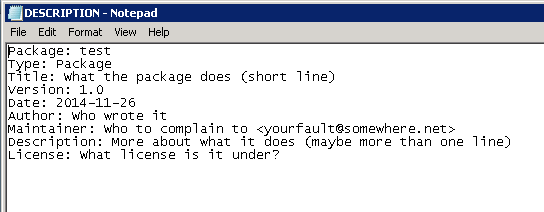
\includegraphics{description.png}
\end{figure}
The lines that need to be edited are the Title, Author, Maintainer, Description, and License. If your package depends on another package (say you write a function that can handle \texttt{Surv} variables, for survival analysis, and thus depends on the \texttt{survival} package) the convention is to add a line titled Imports after the Description line. In the case where we needed the \texttt{survival} package, we would write ``Imports: survival''. This line ensures that if the required packages are not loaded, R will throw an error when the user attempts to load \texttt{test}.
\clearpage
\subsection{The \texttt{NAMESPACE} file}
The second file created is the \texttt{NAMESPACE} file. This file controls which functions are imported or exported by the package. Initially, it looks like Figure \ref{namespace}.
\begin{figure}[h]
\caption{The \texttt{NAMESPACE} file}
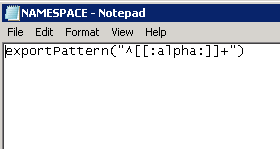
\includegraphics{namespace.png}
\label{namespace}
\end{figure}
This initial line tells the package to export all of the files that have a corresponding help file. If you need to export additional functions, write ``export(functionname)''. If you need to import functions (for example, from the \texttt{survival} package as above) write ``import(functionname)'' to import specific functions or ``import(packagename)'' to import all functions from a package. This file and the \texttt{DESCRIPTION} file MUST be in the package folder, or else it cannot be built.

\subsection{The \texttt{Read-and-delete-me} file}
The last file created in the main package folder is the \texttt{Read-and-delete-me} file (Figure \ref{read-and-delete}). It tells you the most basic items to complete before your package can be built.
\begin{figure}[h]
\caption{The \texttt{Read-and-delete-me} file}
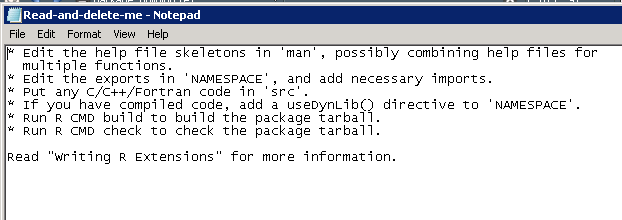
\includegraphics{read-and-delete.png}
\label{read-and-delete}
\end{figure}
This file MUST be deleted before the package can be built.
\clearpage
\subsection{The \texttt{man} files}
Navigate to the package directory. Notice that there is a subfolder titled ``man''. This contains the skeleton of the help manual files for each function in your package. In our case, this folder contains three files: \texttt{descrip}, \texttt{mri}, and \texttt{test-package}. All three of these files must be edited before we can build. If you open up the \texttt{descrip} file, the first few lines will look like Figure \ref{descripman}.
\begin{figure}[h]
\caption{Sample Manual File}
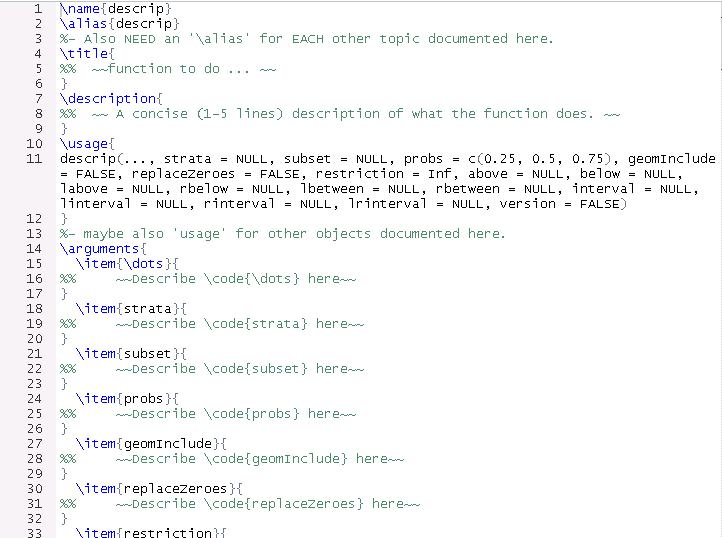
\includegraphics[scale=.8]{descrip_man.png}
\label{descripman}
\end{figure}
The second item in the file is titled \texttt{alias}. For those who have many functions in their package, but only want the user to have access to a few of them, this line allows the package to pass the check command. If you only want the user to use a few functions, you can delete the \texttt{man} files for your hidden functions and add them as aliases to the \texttt{man} file that they are associated with. For example, if we had a function \texttt{testDescrip} that performed a necessary part of the \texttt{descrip} function but was located in a separate file, we could delete the \texttt{man} file for \texttt{testDescrip} and put \texttt{textDescrip} in the \texttt{alias} line of the \texttt{man} file for \texttt{descrip}.

The \texttt{usage} line shows all of the default values in your R file for \texttt{descrip}. This usually does not need to be edited, but all of the other lines must be. 

\section{Building the Package}
Once you have edited all of the \texttt{man} files, you are almost ready to build the package. First, however, you must install Rtools. This is a package for building R packages, and is available at \texttt{http://cran.r-project.org/bin/windows/Rtools/}. Once you download and run the installer, a wizard window will pop up and guide you through the process. Accepting all of the defaults is fine (unless you want to build R itself, which we generally don't). After Rtools is installed, however, you are not done. For this to work correctly, your \texttt{PATH} variable must be set correctly. To find the \texttt{PATH} variable, go to Control Panel -$>$ System -$>$ Advanced System Settings -$>$ Advanced Tab. Then go to Environment Variables and find PATH, and click Edit. Check to make sure that there are three entries for Rtools: \begin{verbatim}c:\Rtools\bin;c:\Rtools\perl\bin;c:\Rtools\MinGW\bin;\end{verbatim} Make sure that there are no spaces in-between entries. If R is not already in the path, make sure to add an entry for it. In this test case, R is located in \begin{verbatim}
C:\Users\brianw26\R\R-3.1.1\bin\x64
\end{verbatim}
so we add this to the \texttt{PATH} variable. Also, if you do not already have MikTex installed, it is recommended to do so and is located at \texttt{http://miktex.org/download} (this helps create nice pdfs for the help files). 

Now we can build the package. First, open a command prompt session. Navigate to the directory containing the package. Then type
\begin{verbatim}
R CMD build packagename
\end{verbatim}
This will create a tar.gz file. Next, type
\begin{verbatim}
R CMD check packagename_versionnumber.tar.gz
\end{verbatim}
Where the text after \texttt{check} is the name of the tar.gz file created in the first step. This is where most of the problems come in. The \texttt{check} function makes sure that your package will run and that all of the code works properly (especially if you have examples in your \texttt{man} files). Considerable amounts of time may be spent making sure all of the errors go away. However, you may see other flags as well. These do not need to all be taken care of, even if you are submitting to CRAN. Though it is ideal that all of the flags are taken care of, if you have certain functions or \texttt{man} files which raise flags and can justify them to CRAN, you are okay. The flags which are fine are \texttt{WARNING} flags, but only in certain parts (check CRAN documents for which are okay to have). If there are no errors, last run
\begin{verbatim}
R CMD INSTALL --build packagename
\end{verbatim}
which will create a .zip file which can be downloaded and installed by Windows users. A Mac user must build the package on their machine for the proper tar.gz file to be built. 

\section{Updating the Package}
After the initial build of the package, you may add functions or edit existing functions. Then it is necessary to update the package! First, you must edit the \texttt{DESCRIPTION} file to reflect a new version number - while this is not strictly necessary, it is good practice. Second, make sure that you have a \texttt{man} file for each new function you create, or that you update the \texttt{man} file for an updated existing function. Now that you have a folder for the package, simply place the ``.R'' files in the R subfolder of the package and they will be included when the package is updated. Last, run the three commands from the command prompt in the previous section. This will build the new version of the package!
\end{document}
